\documentclass[11pt,aspectratio=169]{beamer}
\usepackage[T1]{fontenc}
\usepackage[italian]{babel}
\graphicspath{{../img/}{../../docs/img/}}
\usepackage{tema-milanrailsim}

\title{Simulazione della rete ferroviaria Lombarda}
\subtitle{Sviluppo del progetto Milan RailSim}
\author{Fabio Compagnoni}
\institute{Sistemi Complessi: Modelli e Simulazione\\Università degli Studi di Milano-Bicocca}
\date{}

\begin{document}

\begin{frame}[plain]
	\titlepage
\end{frame}

\begin{frame}{Perché questo progetto}
	\begin{columns}[T]
		\begin{column}{0.52\textwidth}
			\textbf{\color{mrsAzzurro}Motivazione}
			\begin{itemize}
				\item Analisi dell'infrastruttura e delle prestazioni della rete ferroviaria lombarda
				\item Rete come \alert{sistema complesso}: comportamento \alert{emergente} dall'interazione fra agenti
				\item La rete suburbana può comportarsi come una metropolitana?
				\item Invariando la rete, è possibile aumentare la frequenza dei treni senza peggiorare le prestazioni?
			\end{itemize}
		\end{column}
		\begin{column}{0.42\textwidth}
			\begin{block}{Domanda di ricerca}
				Qual è la frequenza massima sostenibile prima che il ritardo si propaghi?\\
				Quali sono i colli di bottiglia della rete?
				Quanto costa aumentare il servizio?
			\end{block}
		\end{column}
	\end{columns}
\end{frame}

\begin{frame}{Il modello: elementi del sistema}
	\centering\textbf{Sistema multi-agente situato su un grafo}\par\smallskip
	\begin{tikzpicture}[
		entita/.style={draw=none,fill=mrsFondoAzzurro,text width=4.1cm,inner sep=8pt,align=left,
			drop shadow={opacity=0.15,shadow xshift=0.6pt,shadow yshift=-0.8pt}},
		freccia/.style={-{Stealth[length=7pt]},line width=1.6pt},
		etichetta/.style={font=\small,align=center,text=mrsNero}]
		\node[entita] (agenti) at (0,0) {%
			{\usebeamercolor[fg]{structure}\bfseries Agenti}\par\smallskip
			\begin{itemize}
				\item treni
				\item reattivi, stato interno, piano fisso
				\item 12 tipi di treno
			\end{itemize}};
		\node[entita] (ambiente) at (9.1,0) {%
			{\usebeamercolor[fg]{structure}\bfseries Ambiente}\par\smallskip
			\begin{itemize}
				\item rete come grafo
				\item risorse con capienza
				\item scala meso e micro
				\item attivo: concede e regola i conflitti
			\end{itemize}};
		\fill[mrsAzzurro] (agenti.north west) rectangle ([xshift=3pt]agenti.south west);
		\fill[mrsAzzurro] (ambiente.north west) rectangle ([xshift=3pt]ambiente.south west);
		\draw[freccia,mrsAzzurro] ([yshift=0.55cm]agenti.east) -- node[etichetta,above]{azione\\[-2pt]{\scriptsize chiede, occupa, libera i binari}} ([yshift=0.55cm]ambiente.west);
		\draw[freccia,mrsVerdeScuro] ([yshift=-0.55cm]ambiente.west) -- node[etichetta,below]{percezione\\[-2pt]{\scriptsize tratto concesso o negato}} ([yshift=-0.55cm]agenti.east);
	\end{tikzpicture}
	\par\medskip
	\raggedright
	\begin{alertblock}{}
		\textbf{Interazione} fra treni: indiretta, mediata dall'ambiente $\rightarrow$ \textbf{ostruzione}
	\end{alertblock}
\end{frame}

\begin{frame}[label=cadorna]{L'ambiente: la rete come grafo}
	\vspace*{-0.5cm}
	\begin{columns}[T]
		\begin{column}{0.42\textwidth}
			\begin{itemize}\setlength{\itemsep}{0pt}
				\item \textbf{Grafo orientato}
				\begin{itemize}
					\item nodi: inizio, fine, diramazione
					\item link: un verso; lunghezza, velocità massima, capienza
				\end{itemize}
				\item \textbf{Risorse}: link prenotati insieme
				\begin{itemize}
					\item binario di stazione, sezione di blocco, binario unico, gola
					\item libera / in uso / esaurita
				\end{itemize}
				\item \textbf{Scala ibrida}: linee meso, stazioni micro
			\end{itemize}
			\begin{alertblock}{Ambiente}
				\small inaccessibile $\cdot$ deterministico $\cdot$ non episodico $\cdot$ dinamico $\cdot$ discreto e continuo
			\end{alertblock}
		\end{column}
		\begin{column}{0.56\textwidth}
			\centering
			\resizebox{\linewidth}{!}{% Grafo del nodo Milano Cadorna - Milano Domodossola - Milano Bovisa come e' descritto nel modello
% (data/nodes/cadorna-bovisa.json): dieci binari di testa a Cadorna in cinque gruppi, due gole,
% due fasci di due binari, quattro binari passanti a Domodossola, otto a Bovisa in quattro gruppi,
% con gli ingressi dal Passante e da Porta Garibaldi e le uscite verso Saronno e verso Asso.
% Incluso da modello.tex dentro un ambiente figure.
\begin{tikzpicture}[x=0.8cm, y=0.8cm, >=Stealth,
	nodo/.style={circle, draw, fill=white, inner sep=1.2pt},
	snodo/.style={circle, draw, fill=black!70, inner sep=1.8pt},
	link/.style={->, line width=0.5pt},
	bidi/.style={<->, line width=0.5pt},
	riserva/.style={->, line width=0.5pt, dashed, color=black!55},
	stazione/.style={draw=black!45, line width=0.4pt, rounded corners=3pt},
	esterno/.style={rectangle, draw=black!60, fill=white, rounded corners=2pt, inner sep=2.5pt, font=\scriptsize, align=center},
	binario/.style={<->, line width=1.5pt},
	passante/.style={->, line width=1.5pt},
	etichetta/.style={font=\scriptsize, align=center},
	nota/.style={font=\scriptsize, align=left, anchor=west},
	mxp/.style={color=red!70!black},
	saronno/.style={color=blue!65!black},
	asso/.style={color=green!45!black},
	misti/.style={color=orange!85!black},
	essetre/.style={color=violet!80!black},
	tunnel/.style={color=cyan!60!black}]

	% gole: ogni area ombreggiata e' una sola risorsa
	\fill[blue!60!black, opacity=0.10] (1.8,4.7) -- (1.8,-2.45) -- (4.2,3.0) -- cycle;
	\fill[green!45!black, opacity=0.12] (1.8,0.95) -- (1.8,-2.45) -- (4.2,-0.75) -- cycle;
	\fill[black, opacity=0.07] (9.9,-3.05) rectangle (11.2,5.4);
	\fill[black, opacity=0.07] (13.4,-3.05) rectangle (14.6,5.4);

	% riquadri delle tre stazioni
	\draw[stazione] (-0.75,-2.65) rectangle (2.1,4.9);
	\draw[stazione] (6.45,-1.75) rectangle (8.65,4.0);
	\draw[stazione] (11.2,-3.05) rectangle (13.4,5.4);

	% Cadorna: binario k a y = 4.5 - 0.75 (k - 1)
	\foreach \k/\stile in {1/mxp, 2/saronno, 3/saronno, 4/saronno, 5/saronno,
			6/asso, 7/asso, 8/misti, 9/misti, 10/essetre} {
		\pgfmathsetmacro{\y}{4.5 - 0.75 * (\k - 1)}
		\node[nodo] (t\k) at (0,\y) {};
		\node[nodo] (p\k) at (1.8,\y) {};
		\draw[binario, \stile] (t\k) -- (p\k);
		\node[etichetta, anchor=east] at (-0.15,\y) {\k};
	}

	% gole di Cadorna
	\node[snodo] (g1) at (4.2,3.0) {};
	\node[snodo] (g2) at (4.2,-0.75) {};
	\foreach \k in {1,...,5} { \draw[bidi] (p\k) -- (g1); }
	\foreach \k in {6,7} { \draw[bidi] (p\k) -- (g2); }
	\foreach \k in {8,9,10} { \draw[bidi] (p\k) -- (g1); \draw[bidi] (p\k) -- (g2); }

	% Domodossola: quattro binari passanti, uno per verso
	\foreach \k/\y/\stile in {1/3.4/saronno, 2/2.6/saronno, 3/-0.35/asso, 4/-1.15/asso} {
		\node[nodo] (d\k a) at (6.8,\y) {};
		\node[nodo] (d\k b) at (8.3,\y) {};
	}
	\draw[passante, saronno] (d1a) -- (d1b);
	\draw[passante, saronno] (d2b) -- (d2a);
	\draw[passante, asso] (d3a) -- (d3b);
	\draw[passante, asso] (d4b) -- (d4a);
	\node[etichetta] at (7.55,3.67) {1};
	\node[etichetta] at (7.55,2.33) {2};
	\node[etichetta] at (7.55,-0.08) {3};
	\node[etichetta] at (7.55,-1.42) {4};

	% fasci fra Cadorna e Domodossola
	\draw[link] (g1) -- (d1a);
	\draw[link] (d2a) -- (g1);
	\draw[link] (g2) -- (d3a);
	\draw[link] (d4a) -- (g2);

	% Bovisa: otto binari passanti, dispari verso nord e pari verso Milano
	\foreach \k/\y/\stile in {1/4.9/tunnel, 2/4.2/tunnel, 3/3.4/saronno, 4/2.6/saronno,
			5/-0.35/asso, 6/-1.15/asso, 7/-2.0/tunnel, 8/-2.7/tunnel} {
		\node[nodo] (b\k a) at (11.4,\y) {};
		\node[nodo] (b\k b) at (13.2,\y) {};
	}
	\foreach \k/\stile in {1/tunnel, 3/saronno, 5/asso, 7/tunnel} {
		\draw[passante, \stile] (b\k a) -- (b\k b);
	}
	\foreach \k/\stile in {2/tunnel, 4/saronno, 6/asso, 8/tunnel} {
		\draw[passante, \stile] (b\k b) -- (b\k a);
	}
	\foreach \k/\y in {1/5.15, 3/3.65, 5/-0.1, 7/-1.75} {
		\node[etichetta] at (12.3,\y) {\k};
	}
	\foreach \k/\y in {2/3.95, 4/2.35, 6/-1.4, 8/-2.95} {
		\node[etichetta] at (12.3,\y) {\k};
	}

	% fasci fra Domodossola e Bovisa
	\draw[link] (d1b) -- (b3a);
	\draw[link] (b4a) -- (d2b);
	\draw[link] (d3b) -- (b5a);
	\draw[link] (b6a) -- (d4b);
	\draw[riserva] (d1b) -- (b5a);
	\draw[riserva] (b6a) -- (d2b);

	% ingressi da sud: Passante e Porta Garibaldi
	\node[esterno] (s1) at (7.55,5.95) {Lancetti (Passante)\\e Porta Garibaldi};
	\node[esterno] (s2) at (7.55,-3.3) {Lancetti (Passante)};
	\draw[link] (s1) -- (b1a);
	\draw[link] (b2a) -- (s1);
	\draw[link] (s2) -- (b7a);
	\draw[link] (b8a) -- (s2);

	% uscite a nord: ramo di Saronno e ramo di Asso
	\node[snodo] (ns) at (14.6,3.75) {};
	\node[snodo] (na) at (14.6,-1.55) {};
	\foreach \k in {1,3} { \draw[link] (b\k b) -- (ns); }
	\foreach \k in {2,4} { \draw[link] (ns) -- (b\k b); }
	% i binari 5 e 6 sono del ramo di Asso: verso Saronno sono la riserva
	\draw[riserva] (b5b) to[bend right=14] (ns);
	\draw[riserva] (ns) to[bend left=30] (b6b);
	\foreach \k in {5,7} { \draw[link] (b\k b) -- (na); }
	\foreach \k in {6,8} { \draw[link] (na) -- (b\k b); }
	\draw[bidi] (ns) -- (15.5,3.75);
	\draw[bidi] (na) -- (15.5,-1.55);
	\node[nota] at (15.55,3.75) {Quarto Oggiaro,\\Bollate, Saronno};
	\node[nota] at (15.55,-1.55) {Affori\\(ramo di Asso)};

	% titoli
	\node[etichetta] at (0.7,5.45) {\textbf{Milano Cadorna}\\10 binari di testa};
	\node[etichetta] at (7.55,4.5) {\textbf{Milano Domodossola}\\4 binari passanti};
	\node[etichetta] at (12.3,5.95) {\textbf{Milano Bovisa}\\8 binari passanti};
	\node[etichetta] at (10.55,-3.35) {gola sud};
	\node[etichetta] at (14.0,-3.35) {gola nord};
	\node[etichetta] at (3.4,4.3) {gola f1\\650 m, 30 km/h};
	\node[etichetta] at (3.9,-2.35) {gola f2\\650 m, 30 km/h};
	\node[etichetta] at (5.6,2.0) {fascio f1\\1,6 km};
	\node[etichetta] at (5.9,-1.75) {fascio f2\\1,6 km};
	\node[etichetta] at (9.1,3.65) {2,4 km};

	% legenda
	\begin{scope}[yshift=-3.75cm]
		\draw[binario, mxp] (0,0) -- (0.9,0);
		\node[nota] at (1.0,0) {Cadorna 1: Malpensa Express};
		\draw[binario, saronno] (6.6,0) -- (7.5,0);
		\node[nota] at (7.6,0) {ramo di Saronno};
		\draw[binario, asso] (12.0,0) -- (12.9,0);
		\node[nota] at (13.0,0) {ramo di Asso};
		\draw[binario, misti] (0,-0.6) -- (0.9,-0.6);
		\node[nota] at (1.0,-0.6) {Cadorna 8--9: variabili};
		\draw[binario, essetre] (6.6,-0.6) -- (7.5,-0.6);
		\node[nota] at (7.6,-0.6) {Cadorna 10: S3};
		\draw[binario, tunnel] (12.0,-0.6) -- (12.9,-0.6);
		\node[nota] at (13.0,-0.6) {Passante};
		\fill[black, opacity=0.12] (0,-1.4) rectangle (0.9,-1.0);
		\node[nota] at (1.0,-1.2) {gola: una sola risorsa};
		\draw[riserva] (6.6,-1.2) -- (7.5,-1.2);
		\node[nota] at (7.6,-1.2) {collegamento di riserva};
	\end{scope}
\end{tikzpicture}
}\\
			{\scriptsize\color{mrsNero!65}Esempio: nodo Cadorna -- Domodossola -- Bovisa}
		\end{column}
	\end{columns}
\end{frame}

\begin{frame}{L'agente: il treno}
	\begin{columns}[T]
		\begin{column}{0.46\textwidth}
			\textbf{\color{mrsAzzurro}Proprietà}\par\medskip
			\begin{tabular}{@{}ll@{}}
				\toprule
				Situato & \si{} posizione sul grafo \\
				Reattivo & \si{} stato dei binari \\
				Autonomo & in parte: solo il moto \\
				Proattivo & \no{} \\
				Sociale & \no{} \\
				\bottomrule
			\end{tabular}
			\begin{alertblock}{}
				Reattivo con stato interno $\cdot$ non deliberativo $\cdot$ eterogeneo: 12 tipi di treno con prestazioni diverse
			\end{alertblock}
		\end{column}
		\begin{column}{0.5\textwidth}
			\textbf{\color{mrsAzzurro}Che cosa descrive un treno}
			\begin{itemize}
				\item \textbf{Attributi}: dipendono dal tipo di treno
				\item \textbf{Stato}: posizione di testa e coda, velocità, tratto autorizzato, ritardo
				\item \textbf{Piano}: corse, percorso, fermate e binari, orari; fissato prima della simulazione
				\item \textbf{Recupero energia in frenata} (solo elettrici): energia restituita alla linea e usata dai treni vicini, entro 10 km
			\end{itemize}
		\end{column}
	\end{columns}
\end{frame}

\begin{frame}{Il comportamento: comunicazione treno -- ambiente}
	\centering
	{\small\color{mrsNero!65}Piano di ogni treno (orari, binari) calcolato prima della simulazione}\par\smallskip
	\begin{tikzpicture}[
		entita/.style={draw=none,fill=mrsFondoAzzurro,text width=4.4cm,inner sep=8pt,align=left,
			drop shadow={opacity=0.15,shadow xshift=0.6pt,shadow yshift=-0.8pt}},
		freccia/.style={-{Stealth[length=7pt]},line width=1.6pt},
		etichetta/.style={font=\small,align=center,text=mrsNero}]
		\node[entita,text width=3.4cm] (treno) at (0,0) {%
			{\usebeamercolor[fg]{structure}\bfseries Treno}\par\smallskip
			a ogni aggiornamento chiede il tratto davanti a sé};
		\node[entita,text width=4.6cm] (ambiente) at (9.0,0) {%
			{\usebeamercolor[fg]{structure}\bfseries Ambiente}\par\smallskip
			decide sullo \textbf{stato}: binari occupati o prenotati, treni in arrivo, ordine delle richieste};
		\fill[mrsAzzurro] (treno.north west) rectangle ([xshift=3pt]treno.south west);
		\fill[mrsAzzurro] (ambiente.north west) rectangle ([xshift=3pt]ambiente.south west);
		\draw[freccia,mrsAzzurro] ([yshift=0.45cm]treno.east) -- node[etichetta,above]{richiesta: tratto per arrestarsi\\[-1pt]$s = v^2/2d$} ([yshift=0.45cm]ambiente.west);
		\draw[freccia,mrsVerdeScuro] ([yshift=-0.45cm]ambiente.west) -- node[etichetta,below]{risposta: distanza concessa\\[-1pt]e velocità consentita} ([yshift=-0.45cm]treno.east);
	\end{tikzpicture}
	\par\smallskip
	\raggedright
	\begin{columns}[T]
		\begin{column}{0.46\textwidth}
			\si{} \textbf{concesso} $\rightarrow$ accelera fino alla velocità consentita
		\end{column}
		\begin{column}{0.46\textwidth}
			\no{} \textbf{negato} $\rightarrow$ frena prima del tratto occupato, riprova dopo 10 s
		\end{column}
	\end{columns}
	\vfill
	\begin{alertblock}{}
		Distanza fra i treni: non è un parametro, \textbf{emerge} da velocità e frenata\\
		Tempo: passo di 1 s $\cdot$ eventi ordinati nel passo $\cdot$ risorse in ordine di richiesta
	\end{alertblock}
\end{frame}

\begin{frame}{La ricerca dei dati}
	\centering
	\small
	\begin{tabular}{@{}>{\raggedright}p{3.6cm}>{\raggedright}p{4.8cm}>{\raggedright\arraybackslash}p{4.5cm}@{}}
		\toprule
		\intestazione{Fonte} & \intestazione{Dati} & \intestazione{Nel modello} \\
		\midrule
		Orario GTFS Trenord & fermate, linee, corse, orari & 2501 corse, 61 linee \\[2pt]
		OpenStreetMap & tracciati, lunghezze, velocità, binari & 1157 link su 1179 misurati \\[2pt]
		OpenRailwayMap& binario unico, posti di movimento & 40 tratte, 236 stazioni censite \\[2pt]
		Rilievo dei binari & binari delle stazioni, uso per linea & 180 stazioni binario per binario \\[2pt]
		Schede tecniche dei treni & moto, masse, potenze, posti & 12 tipi di treno \\
		\bottomrule
	\end{tabular}
	\vfill
	\raggedright
	\begin{alertblock}{}
		Risultato: rete di 6008 nodi e 11\,452 link
	\end{alertblock}
\end{frame}

\begin{frame}{Orari: il piano di ogni treno}
	\vspace*{-0.2cm}
	\centering
	\begin{tikzpicture}[
		passo/.style={fill=mrsFondoAzzurro,text width=2.05cm,minimum height=0.9cm,align=center,
			inner sep=4pt,font=\small\bfseries,text=mrsAzzurro,
			drop shadow={opacity=0.15,shadow xshift=0.6pt,shadow yshift=-0.8pt}},
		nota/.style={font=\scriptsize,text=mrsNero!70,align=center,text width=2.3cm},
		freccia/.style={-{Stealth[length=5pt]},line width=1.2pt,mrsVerde}]
		\foreach \testo/\sotto [count=\i] in {Orario GTFS/{},Corse del giorno/2501 corse,Treni alle corse/370 treni,Binari/in ordine di tempo,Ricoveri/sosta > 60 min} {
			\node[passo] (p\i) at ({(\i-1)*2.75},0) {\testo};
			\node[nota,below=2pt of p\i] {\sotto};
		}
		\foreach \i [evaluate=\i as \j using int(\i+1)] in {1,...,4} {
			\draw[freccia] (p\i) -- (p\j);
		}
	\end{tikzpicture}
	\par\smallskip
	\raggedright
	\small
	\begin{tabular}{@{}>{\bfseries\color{mrsAzzurro}}l>{\raggedright\arraybackslash}p{11.3cm}@{}}
		Corse & corse del giorno dal GTFS; ogni fermata con attesa dell'orario di partenza \\[2pt]
		Treni & turni: al capolinea il treno fa la corsa successiva della linea, dopo 5 min di inversione \\[2pt]
		Tipo di treno & quote per linea, distribuite in modo uniforme; il treno mantiene il tipo per tutto il turno \\[2pt]
		Binari & piano dei binari in ordine di tempo: primo binario ammesso libero per tutta la sosta \\[2pt]
		Ricoveri & soste oltre 60 min al ricovero, rientro 4 min prima della partenza \\
	\end{tabular}
	\vfill
	\begin{alertblock}{}
		Durante la simulazione il piano non cambia: solo deviazione su un altro binario della stessa stazione, se quello previsto è occupato
	\end{alertblock}
\end{frame}

\begin{frame}{Le stazioni}
	\vspace*{-0.4cm}
	\begin{columns}[T]
		\begin{column}{0.56\textwidth}
			\textbf{\color{mrsAzzurro}Composizione}
			\begin{itemize}
				\item \textbf{Gole}: deviatoi di ingresso e uscita, una sola risorsa
				\item \textbf{Binari} in gruppi: passanti $\cdot$ di testa $\cdot$ misti
				\item \textbf{Ricovero}: soste oltre 60 min
			\end{itemize}
		\end{column}
		\begin{column}{0.4\textwidth}
			\textbf{\color{mrsAzzurro}Stazioni di dettaglio: 180}\par\smallskip
			\begin{tabular}{@{}lr@{}}
				\toprule
				Nodo di Milano e Passante & 16 \\
				Diramazioni e capolinea & 27 \\
				Linee a binario unico & 137 \\
				\bottomrule
			\end{tabular}\par\medskip
			{\small\hyperlink{cadorna}{\color{mrsAzzurro}$\rightarrow$ Esempio: nodo Cadorna -- Bovisa}}
		\end{column}
	\end{columns}
	\vfill
	\begin{block}{Assegnazione dei binari}
		\begin{itemize}
			\item \textbf{per verso}: binari dedicati a una direzione di marcia
			\item \textbf{per linea}: gruppi o binario fisso (es.\ Cadorna 1: Malpensa Express)
			\item \textbf{libera}: qualunque binario del gruppo, purché non contromano
		\end{itemize}
		{\small sempre: collegato a provenienza e destinazione $\cdot$ libero per tutta la sosta}
	\end{block}
\end{frame}

\begin{frame}[squeeze]{Railsim e le aggiunte del progetto}
	\vspace*{-0.4cm}
	\begin{columns}[T]
		\begin{column}{0.47\textwidth}
			\textbf{\color{mrsAzzurro}railsim}\\
			{\small\color{mrsNero!65}estensione ferroviaria di MATSim}
			\small
			\begin{itemize}
				\item motore secondo per secondo
				\item moto: accelerazione, frenata, velocità massima per tipo
				\item risorse con capienza; binario unico come risorsa condivisa
				\item prenotazione $s = v^2/2d$
				\item scala meso, micro o mista
				\item punti di estensione: disposizione dei treni, prevenzione degli stalli
			\end{itemize}
			\begin{alertblock}{}
				Nessuna modifica al codice di railsim: solo i suoi punti di estensione
			\end{alertblock}
		\end{column}
		\begin{column}{0.5\textwidth}
			\textbf{\color{mrsAzzurro}Aggiunte del progetto}
			\small
			\begin{itemize}
				\item \textbf{Rete}: GTFS + OpenStreetMap, 180 stazioni di dettaglio
				\item \textbf{Piano}: corse, turni, tipi di treno, binari, ricoveri
				\item \textbf{Gestore delle risorse}: qualunque binario libero in stazione
				\item \textbf{Prevenzione degli stalli} sul binario unico: blocchi fra incroci, consenso all'ingresso
				\item \textbf{Deviazioni}: solo fra binari collegati, senza saltare fermate
				\item \textbf{Misure}: puntualità, energia, costi
				\item \textbf{Scenari} e applicazione grafica
			\end{itemize}
		\end{column}
	\end{columns}
\end{frame}

\begin{frame}{Gli scenari}
	\vspace*{-0.4cm}
	\textbf{Caso base}: orario reale, riferimento e validazione\par\medskip
	\centering
	\small
	\begin{tabular}{@{}l>{\raggedright}p{5cm}>{\raggedright\arraybackslash}p{5cm}@{}}
		\toprule
		& \intestazione{Passante ad alta frequenza} & \intestazione{Potenziamento per linea} \\
		\midrule
		Obiettivo & aumentare il servizio sui tratti urbani & individuare i colli di bottiglia della rete \\
		Parametro & attesa massima 15 o 10 min & attesa per percorso, 3--30 min \\
		Dove & tratti urbani, 4 relazioni & intera linea \\
		Quando & punta feriale & tutto il giorno \\
		Distanza minima & 300 s; tunnel 180 s & nessuna \\
		Corse in conflitto & scartate & inserite e segnalate \\
		\bottomrule
	\end{tabular}
	\vfill
	\raggedright
	\begin{alertblock}{}
		Corse aggiunte = copie di corse reali nei vuoti dell'orario; cambia solo l'orario, tutto il resto resta fisso
	\end{alertblock}
\end{frame}

\begin{frame}{Demo}
	\begin{columns}[c]
		\begin{column}{0.6\textwidth}
			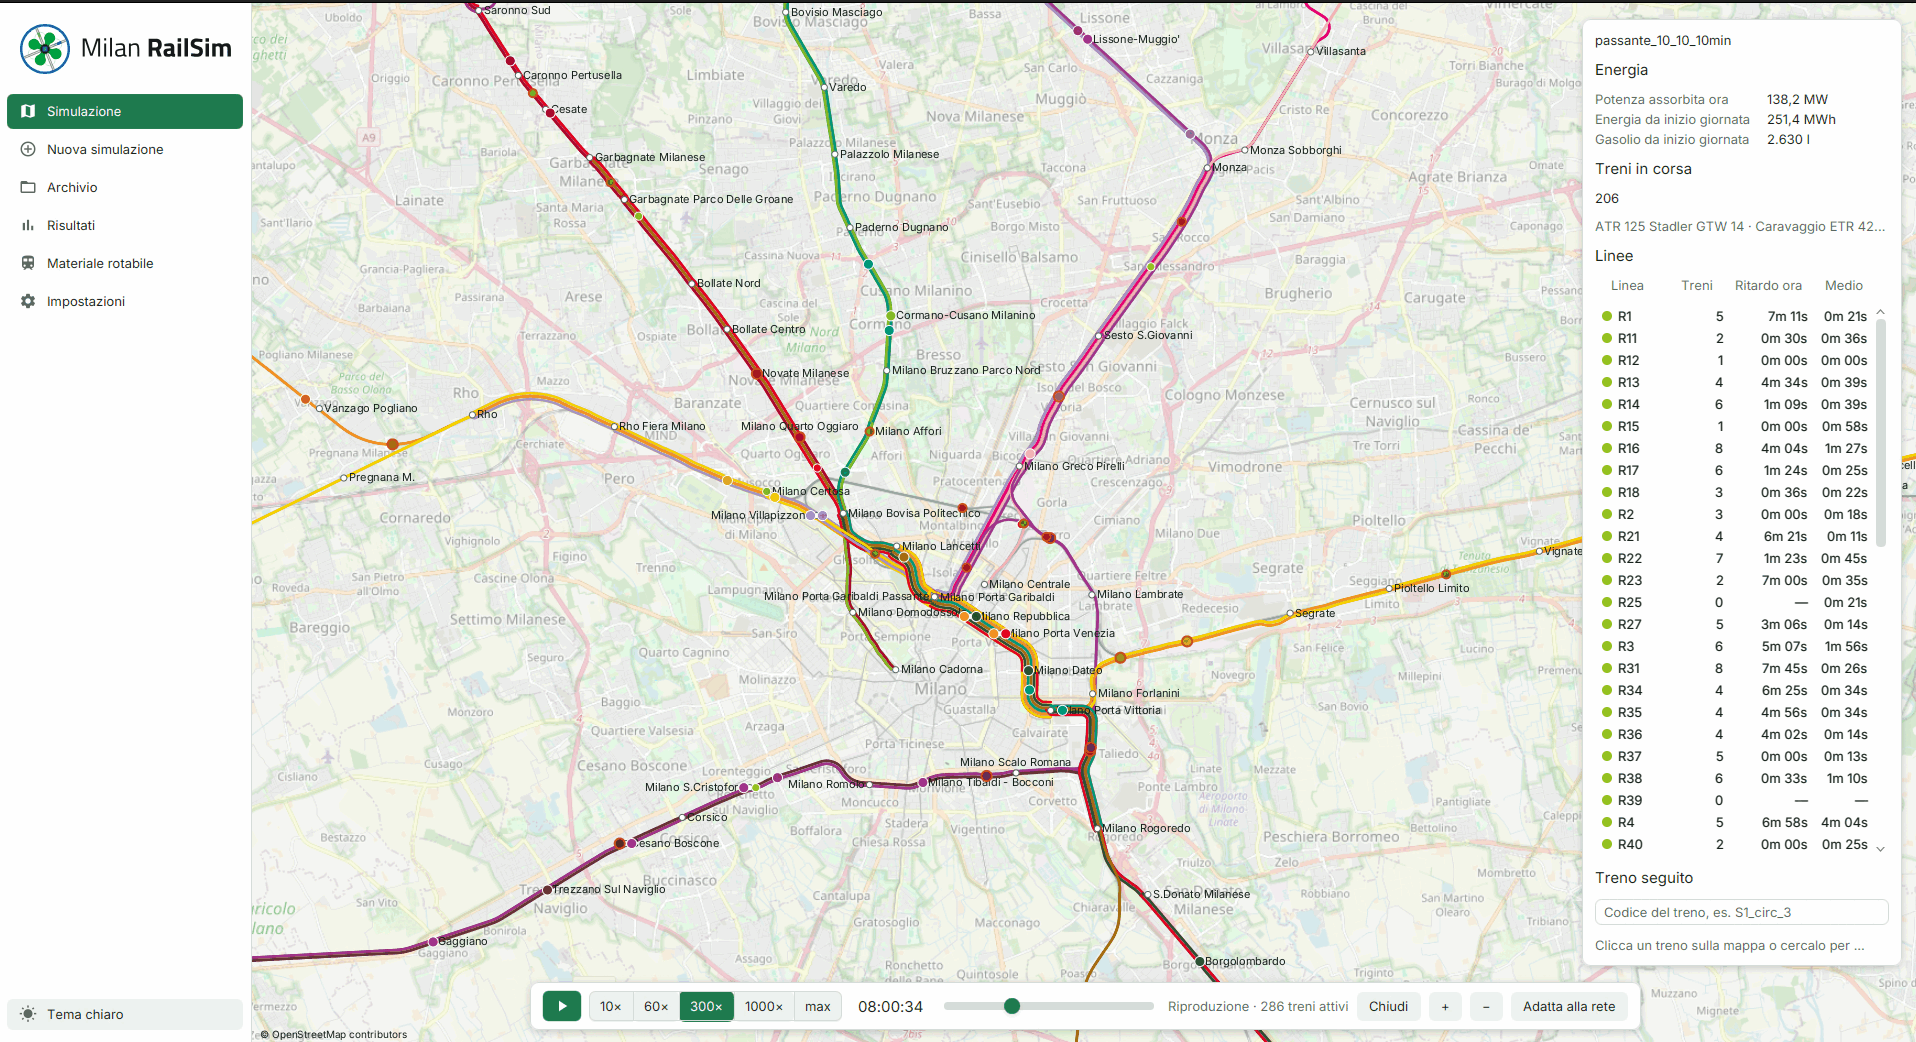
\includegraphics[width=\linewidth]{run-milano.png}
		\end{column}
		\begin{column}{0.37\textwidth}
			\begin{enumerate}
				\item \textbf{Nuova simulazione}: giorno, scenario, anteprima delle corse aggiunte
				\item \textbf{Mappa}: treni in tempo reale, linee, ritardi, treno seguito
				\item \textbf{Risultati}: puntualità, energia, costi, flotta
				\item \textbf{Archivio}: confronto fra due simulazioni
			\end{enumerate}
		\end{column}
	\end{columns}
\end{frame}

\begin{frame}[squeeze]{Come leggere i dati}
	\vspace*{-0.4cm}
	\begin{columns}[T]
		\begin{column}{0.5\textwidth}
			\textbf{\color{mrsAzzurro}Indicatori}
			\small
			\begin{itemize}
				\item \textbf{Regolarità}: corse completate / corse programmate
				\begin{itemize}
					\item corsa completata, interrotta o mai partita
				\end{itemize}
				\item \textbf{Puntualità}: arrivi con ritardo $\le$ 5 min, a destinazione e su tutte le fermate
				\item \textbf{Ritardo}: solo la parte positiva; medio e 95° percentile
				\item \textbf{Treni utilizzati} e massimo in corsa insieme: flotta necessaria
				\item \textbf{Energia} e \textbf{costo}: da orario e simulato
			\end{itemize}
		\end{column}
		\begin{column}{0.46\textwidth}
			\textbf{\color{mrsAzzurro}Grafici}
			\small
			\begin{itemize}
				\item \textbf{Ritardo per ora}: dove si accumula nella giornata
				\item \textbf{Distribuzione degli scostamenti}: anticipi ($<0$) e ritardi ($>0$)
				\item \textbf{Treni in corsa per ora e per tipo}: punte del servizio, flotta usata
				\item \textbf{Potenza}: assorbita e recuperata in frenata
				\item \textbf{Spazio-tempo} di una linea: slide successiva
			\end{itemize}
			\begin{alertblock}{}
				Contano le differenze fra scenari, non i valori assoluti
			\end{alertblock}
		\end{column}
	\end{columns}
\end{frame}

\begin{frame}{Il diagramma spazio-tempo}
	\vspace*{-0.3cm}
	\begin{columns}[T]
		\begin{column}{0.42\textwidth}
			\centering
			\begin{tikzpicture}[x=0.55cm,y=0.5cm,
				treno/.style={line width=1.6pt,line cap=round},
				nota/.style={font=\scriptsize,text=mrsNero!80,align=left}]
				\draw[-{Stealth[length=5pt]},mrsNero!70] (0,0) -- (8.3,0) node[below left,font=\scriptsize] {ora};
				\draw[-{Stealth[length=5pt]},mrsNero!70] (0,0) -- (0,6.3) node[above right,font=\scriptsize] {km};
				% treno A: in moto, sosta, in moto
				\draw[treno,mrsAzzurro] (0.3,0) -- (2,2.5) -- (3,2.5) -- (4.6,5.8);
				% treno B: raggiunge A, attende in coda, riparte
				\draw[treno,mrsVerdeScuro] (1.6,0) -- (2.8,1.9) -- (3.8,1.9) -- (5.6,5.8);
				% treno C: si ferma e non arriva
				\draw[treno,mrsGrigio!70!black] (4.6,0) -- (6.2,2.6) -- (7.6,2.6);
				\node[font=\bfseries\color{red!70!black}] at (7.6,2.6) {$\times$};
				\node[nota,anchor=east] at (3.6,4.4) {in moto};
				\node[nota,anchor=south] at (2.5,2.6) {sosta};
				\node[nota,anchor=north] at (3.3,1.8) {coda};
				\node[nota,anchor=north] at (6.9,2.4) {interrotta};
			\end{tikzpicture}
		\end{column}
		\begin{column}{0.55\textwidth}
			\centering
			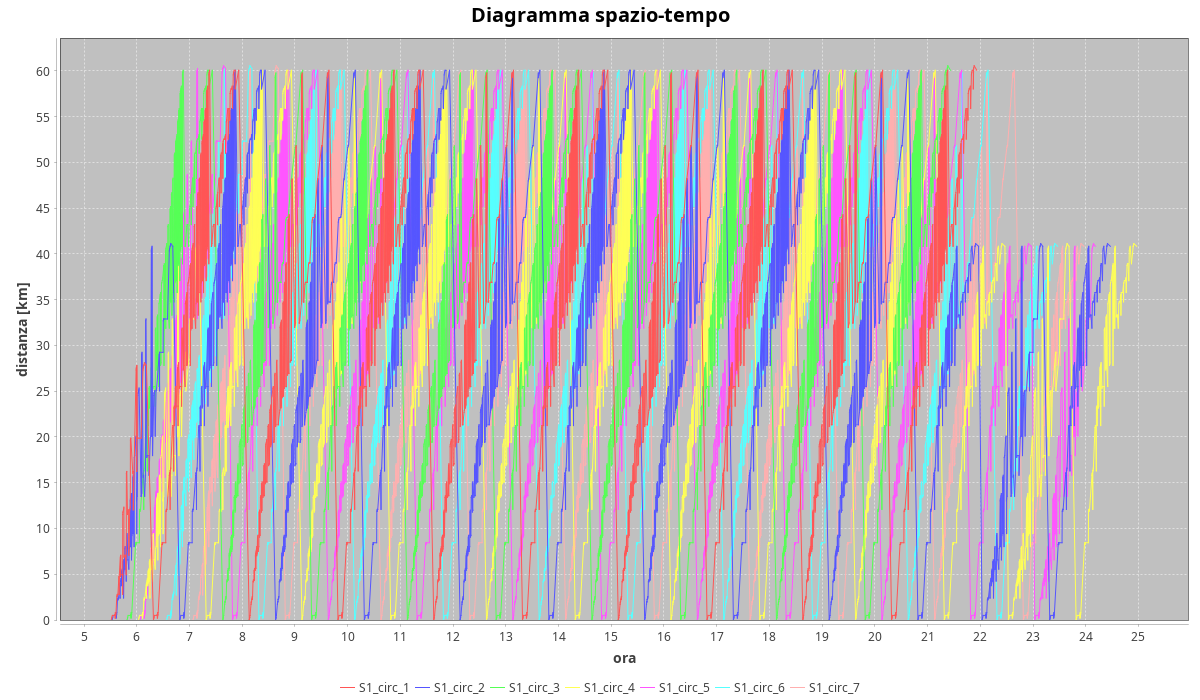
\includegraphics[width=0.9\linewidth]{reale_spazio_tempo.png}\par
			\scriptsize\color{mrsNero!65}Linea S1, giorno feriale $\cdot$ un colore = un treno
		\end{column}
	\end{columns}
	\vfill
	\begin{alertblock}{}
		inclinata = in moto (pendenza = velocità) $\cdot$ orizzontale = fermo $\cdot$ tratto orizzontale subito sotto un'altra linea = coda: il treno attende che il tratto davanti si liberi $\cdot$ linea che non arriva in fondo = corsa interrotta
	\end{alertblock}
\end{frame}

\begin{frame}{I costi: voci e calcolo}
	\centering
	\begin{tikzpicture}[
		card/.style={anchor=north,fill=mrsFondoAzzurro,inner sep=6pt,font=\small,
			drop shadow={opacity=0.15,shadow xshift=0.6pt,shadow yshift=-0.8pt}},
		driver/.style={font=\bfseries,text=mrsAzzurro},
		base/.style={anchor=north,font=\scriptsize,text=mrsNero!70,align=center,text width=3cm}]
		\foreach \x/\nome/\voci/\sotto [count=\i] in {
			0/Tempo/{\textbf{Personale di bordo}\\140 \euro{} a treno-ora\\macchinista + capotreno}/{ore effettive,\\ritardi compresi},
			3.45/Chilometri/{\textbf{Manutenzione}\\2,5 \euro/km\\[3pt]\textbf{Accesso alla rete}\\2,5 \euro/km}/{treni-km},
			6.9/Energia/{\textbf{Elettricità}\\0,10 \euro/kWh\\[3pt]\textbf{Gasolio}\\0,95 \euro/l}/{consumi calcolati\\dal moto},
			10.35/Treni/{\textbf{Materiale rotabile}\\650 \euro{} a treno-giorno}/{treni utilizzati}} {
			\node[card] (c\i) at (\x,0) {\begin{minipage}[t][2.6cm][t]{2.75cm}\raggedright
				{\usebeamercolor[fg]{structure}\bfseries \nome}\par\smallskip \voci\end{minipage}};
			\fill[mrsAzzurro] (c\i.north west) rectangle ([xshift=3pt]c\i.south west);
			\node[base] at ([yshift=-3pt]c\i.south) {\sotto};
		}
	\end{tikzpicture}
	\par\medskip
	\raggedright
	\textbf{Energia}: $F = m \rho a + R(v)$ ogni 5 s $\cdot$ recupero in frenata entro 10 km
	\vfill
	\begin{alertblock}{}
		Costo simulato vs costo da orario: la differenza misura la circolazione perturbata
	\end{alertblock}
\end{frame}

\begin{frame}{Costi per l'aumento del servizio}
	\vspace*{-0.4cm}
	{\small\color{mrsNero!65}Giorno feriale; orario reale: 1\,630\,662 \euro{} al giorno}\par\smallskip
	\centering
	\small
	\begin{tabular}{@{}lrrrrr@{}}
		\toprule
		& \intestazione{Passante 15} & \intestazione{Passante 10} & \intestazione{Caso 1} & \intestazione{Caso 3} & \intestazione{Caso 2} \\
		\midrule
		Corse aggiunte & 47 (+2\%) & 189 (+8\%) & 916 (+37\%) & 1069 (+43\%) & 1359 (+54\%) \\
		Treni in più & 10 & 33 & 146 & 178 & 198 \\
		Costo in più & +1,6\% & +6,2\% & +45\% & +52\% & +64\% \\
		Regolarità & 100\% & 100\% & 95,2\% & 83,4\% & 88,3\% \\
		\bottomrule
	\end{tabular}
	\par\medskip
	\raggedright
	\textbf{Passante 10, per voce}: materiale rotabile +8,9\% $\cdot$ personale +7,4\% (+448 ore al giorno) $\cdot$ elettricità +5,7\% $\cdot$ manutenzione e rete +4,8\%
	\begin{itemize}
		\item treno-km aggiunto: 13,33 \euro{} contro 10,46 \euro{} medi
		\item flotta: 33 treni in più, sulla carta disponibili (TSR 101 su circa 104)
	\end{itemize}
\end{frame}

\begin{frame}{Validazione: il caso base confrontato con Trenord}
	\vspace*{-0.4cm}
	{\small\color{mrsNero!65}Trenord $\rightarrow$ modello}\par\smallskip
	\centering
	\begin{tikzpicture}[
		card/.style={anchor=north,inner sep=6pt,font=\small,
			drop shadow={opacity=0.15,shadow xshift=0.6pt,shadow yshift=-0.8pt}}]
		\foreach \x/\colore/\fondo/\titolo/\testo [count=\i] in {
			0/mrsVerdeScuro/mrsFondoVerde/{\si{} Riprodotto}/{\textbf{Corse in un feriale}\\$>$\,2350 $\rightarrow$ 2501 {\scriptsize(2349 senza TILO)}\\[3pt]\textbf{Tempi di percorrenza}: scarto $<$ 1\%\\[3pt]\textbf{Energia all'anno}\\566 $\rightarrow$ 560--598 GWh\\[3pt]\textbf{Treni}: 456 in flotta $\rightarrow$ 370},
			6.95/mrsAzzurro/mrsFondoAzzurro/{$\approx$ Nel verso atteso}/{\textbf{Puntualità a 5 min}\\92,7\%* $\rightarrow$ 94,4\%\\[3pt]\textbf{Regolarità}\\circa 96,7\% $\rightarrow$ 100\%\\[3pt]{\color{mrsNero!70}niente guasti, soppressioni, passeggeri}}} {
			\node[card,fill=\fondo] (v\i) at (\x,0) {\begin{minipage}[t][3.3cm][t]{6cm}\raggedright
				{\color{\colore}\bfseries \titolo}\par\smallskip \testo\end{minipage}};
			\fill[\colore] (v\i.north west) rectangle ([xshift=3pt]v\i.south west);
		}
	\end{tikzpicture}\par
	\raggedright
	{\scriptsize\color{mrsNero!65}* sole cause imputabili all'operatore (83,8\% con tutte le cause)}
	\vfill
	\begin{alertblock}{}
		Attendibili le differenze fra scenari; puntualità e regolarità sono un limite superiore
	\end{alertblock}
	{\scriptsize\color{mrsNero!65}Fonti: Trenord, Bilancio di Sostenibilità 2025; Carta dei Servizi 2024 $\cdot$ indicatori: delibera ART 16/2018}
\end{frame}

\begin{frame}{Conclusioni}
	\vspace*{-0.2cm}
	\centering
	\begin{tikzpicture}[
		card/.style={anchor=north,fill=mrsFondoAzzurro,inner sep=6pt,font=\small,
			drop shadow={opacity=0.15,shadow xshift=0.6pt,shadow yshift=-0.8pt}}]
		\foreach \x/\titolo/\testo [count=\i] in {
			0/{Quanta frequenza?}/{\si{} 10 min sui tratti urbani, in punta\\[2pt]\no{} +37\% di corse su tutta la rete\\[2pt]{\color{mrsNero!70}fra +8\% e +37\%: soglia non misurata}},
			4.65/{Quali colli di bottiglia?}/{binario unico: S9, Cremona, Valtellina\\[2pt]tunnel del Passante e nodi dove le linee terminano},
			9.3/{Quanto costa?}/{+6,2\% al giorno\\[2pt]33 treni in più, nella flotta\\[2pt]+448 ore di personale al giorno}} {
			\node[card] (k\i) at (\x,0) {\begin{minipage}[t][2.95cm][t]{3.9cm}\raggedright
				{\usebeamercolor[fg]{structure}\bfseries \titolo}\par\smallskip \testo\end{minipage}};
			\fill[mrsAzzurro] (k\i.north west) rectangle ([xshift=3pt]k\i.south west);
		}
		\node[anchor=north west,inner sep=0pt,font=\small\bfseries,text=mrsAzzurro] (titolo) at ([yshift=-0.3cm]k1.south west) {Obiettivi};
		\coordinate (o0) at ([yshift=-0.15cm]titolo.south west);
		\foreach \esito/\nome [count=\i, evaluate=\i as \prima using int(\i-1)] in {
			\si{}/modello di base validato,
			\si{}/scenario urbano,
			$\approx$/scenario su tutta la rete,
			$\approx$/costi} {
			\ifnum\i=1
				\node[anchor=north west,fill=mrsFondoAzzurro,inner sep=4pt,font=\small] (o\i) at (o0) {\esito{} \nome};
			\else
				\node[right=8pt of o\prima,fill=mrsFondoAzzurro,inner sep=4pt,font=\small] (o\i) {\esito{} \nome};
			\fi
		}
	\end{tikzpicture}
	\par\medskip
	\raggedright
	\begin{alertblock}{}
		Il servizio può crescere solo in modo localizzato: il primo limite è il binario unico, poi il Passante con i suoi nodi
	\end{alertblock}
\end{frame}

\begin{frame}{Limiti e sviluppi}
	\vspace*{-0.4cm}
	\centering
	\small
	\begin{tabular}{@{}>{\raggedright}p{6cm}c>{\raggedright\arraybackslash}p{6cm}@{}}
		\toprule
		\intestazione{Limite del modello} & & \intestazione{Sviluppo} \\
		\midrule
		Deterministico: niente guasti né ritardi casuali & {\color{mrsVerde}$\rightarrow$} & perturbazioni casuali e repliche \\[3pt]
		Oltre la soglia nessuno regola la circolazione: i treni si bloccano & {\color{mrsVerde}$\rightarrow$} & regolazione della circolazione: precedenze, trattenimento, soppressioni \\[3pt]
		Senza passeggeri: soste fisse & {\color{mrsVerde}$\rightarrow$} & passeggeri come agenti \\[3pt]
		Solo treni Trenord & {\color{mrsVerde}$\rightarrow$} & treni delle altre imprese nei nodi \\[3pt]
		Velocità sempre massima & {\color{mrsVerde}$\rightarrow$} & profilo di velocità adattivo \\[3pt]
		Binario unico come limite & {\color{mrsVerde}$\rightarrow$} & simulare il raddoppio selettivo \\
		\bottomrule
	\end{tabular}
	\vfill
	\raggedright
	\begin{alertblock}{}
		Passaggi a livello e pendenze non rappresentati
	\end{alertblock}
\end{frame}

\end{document}